\section{Conclusion and Future Work}
\label{sec:conclusion}


\subsection{Summary of Contributions}
This project provides a comprehensive empirical and theoretical exploration of diversity and aggregation in ensemble learning, with a specific focus on Negative Correlation Learning and its extensions. The findings demonstrate that diversity is a double-edged sword: when carefully managed, it enhances predictive accuracy while reducing resource requirements; however, if left uncontrolled, an ensemble can actually underperform relative to a single model. The primary contributions are as follows: 
\begin{enumerate}
    \item \textbf{Theoretical Bridging} \\
    The work establishes a clear link between ensemble parameters (e.g. ensemble size and model complexity) and overall performance. By using diversity as a central explanatory variable, the project clarifies how these attributes influence ensemble MSE. 

    \item \textbf{Validation of Ensemble Utility} \\
    The research reinforces the fundamental advantages of ensemble methods over single-model approaches, providing both mathematical evidence and empirical validation of their superior predictive power and resource efficiency. 

    \item \textbf{Exploration of Diversity at Multiple Dimensions} \\
    The research moves beyond weight-based diversity and explores the impact of architectural diversity on performance in ensemble learning. NEAT is combined with NCL, which also allows for the evolutionary discovery of the optimal model structures and $\lambda$ for the regression task. 

    \item \textbf{Algorithmic Innovation} \\
    A key technical contribution is the development of an algorithm that converts dynamic neural networks into a GPU-compatible format. This implementation significantly increases computational efficiency and provides a substantial performance boost for modern machine learning workflows. 

    \item \textbf{Recursive Ensemble Framework} \\
    We introduced the concept of recursive ensemble models, demonstrating that significant performance gains are achievable when utilising optimal aggregator-arrangement pairings. This provides a novel foundation for future research into hierarchical ensemble architectures. 
\end{enumerate}


\subsection{Potential Improvements}
\paragraph{Repeating experiment}
Experiments were not repeated to reduce computational cost. Although repetition could mitigate noise, this project prioritised exploring a wider range of ensemble behaviours. The resulting noise was considered acceptable as key patterns remained observable. 

\paragraph{More thorough hyperparameter tuning}
Hyperparameter tuning was applied only to critical parameters (e.g. $\lambda$) while others used default values (e.g. $learning\_rate = 0.001$). Although further tuning could be performed, the limited number and lower impact of these parameters made this approach sufficient for the study. 

\paragraph{More variety of datasets and problems}
All experiments were conducted using the Boston Housing dataset, a standard regression benchmark. While the observed behaviours are inherently tied to this specific data distribution, future work can involve testing datasets with diverse characteristics, such as varying sample sizes and problem types, to uncover broader ensemble trends and effects of diversity. Additionally, removing the regression constraint would allow for the exploration of different aggregation mechanisms, such as majority voting for classification tasks. 


\subsection{Future Research Directions}
\paragraph{Double descent in ensemble MSE and $\rho$}
As mentioned in Section~\ref{subsec:evaluation_ncl}, an interesting and unexpected phenomenon of double descents in ensemble MSE and $\rho$ had occurred when $\lambda$ reached extreme values. Further empirical studies to explain such behaviour could be attempted. 

\paragraph{Reversible algorithm to run dynamic neural networks on GPU}
As mentioned in Section~\ref{subsubsec:dynamic_nn_on_gpu}, the algorithm proposed can only convert dynamic neural networks from a DAG to a fully-connected graph. Thus, it fails when there is backpropagation and cannot be used in training. Future development of converting a fully-connected graph to a DAG is beneficial as it provides huge performance boost for training any NEAT models. 

\paragraph{More diverse recursive ensemble models}
Recursive ensemble models composed of different types of base learners could be explored with additional time. For example, one base learner in the recursive model could be an arithmetic-mean-ensemble while the two base learners could be a NCL ensemble model and a recursive NEAT-NCL ensemble model respectively. 

Furthermore, more variations in ensemble architecture could be included in the experiment. In this experiment, all base learners either formed a tree-shape or were either at the same depth as shown in Figure~\ref{fig:recursive_perfect_binary_tree} and Figure~\ref{fig:recursive_flat_tree}. Architectures shown in Figure~\ref{fig:recursive_tree_potential_1} and Figure~\ref{fig:recursive_tree_potential_2} could be also attempted to investigate the best ensemble architecture for this problem. 

Lastly, each MLP was fixed to have 1 hidden layer of 6 hidden nodes in Section~\ref{subsec:stage_6}. Other MLP architectures, e.g. 1 hidden layer of 2 or 12 hidden nodes, could be attempted. 

% 2 Image
\begin{figure}[H]
    \centering

    \begin{minipage}[t]{0.48\textwidth}
        \capstart
        \vspace{0pt}
        \centering
        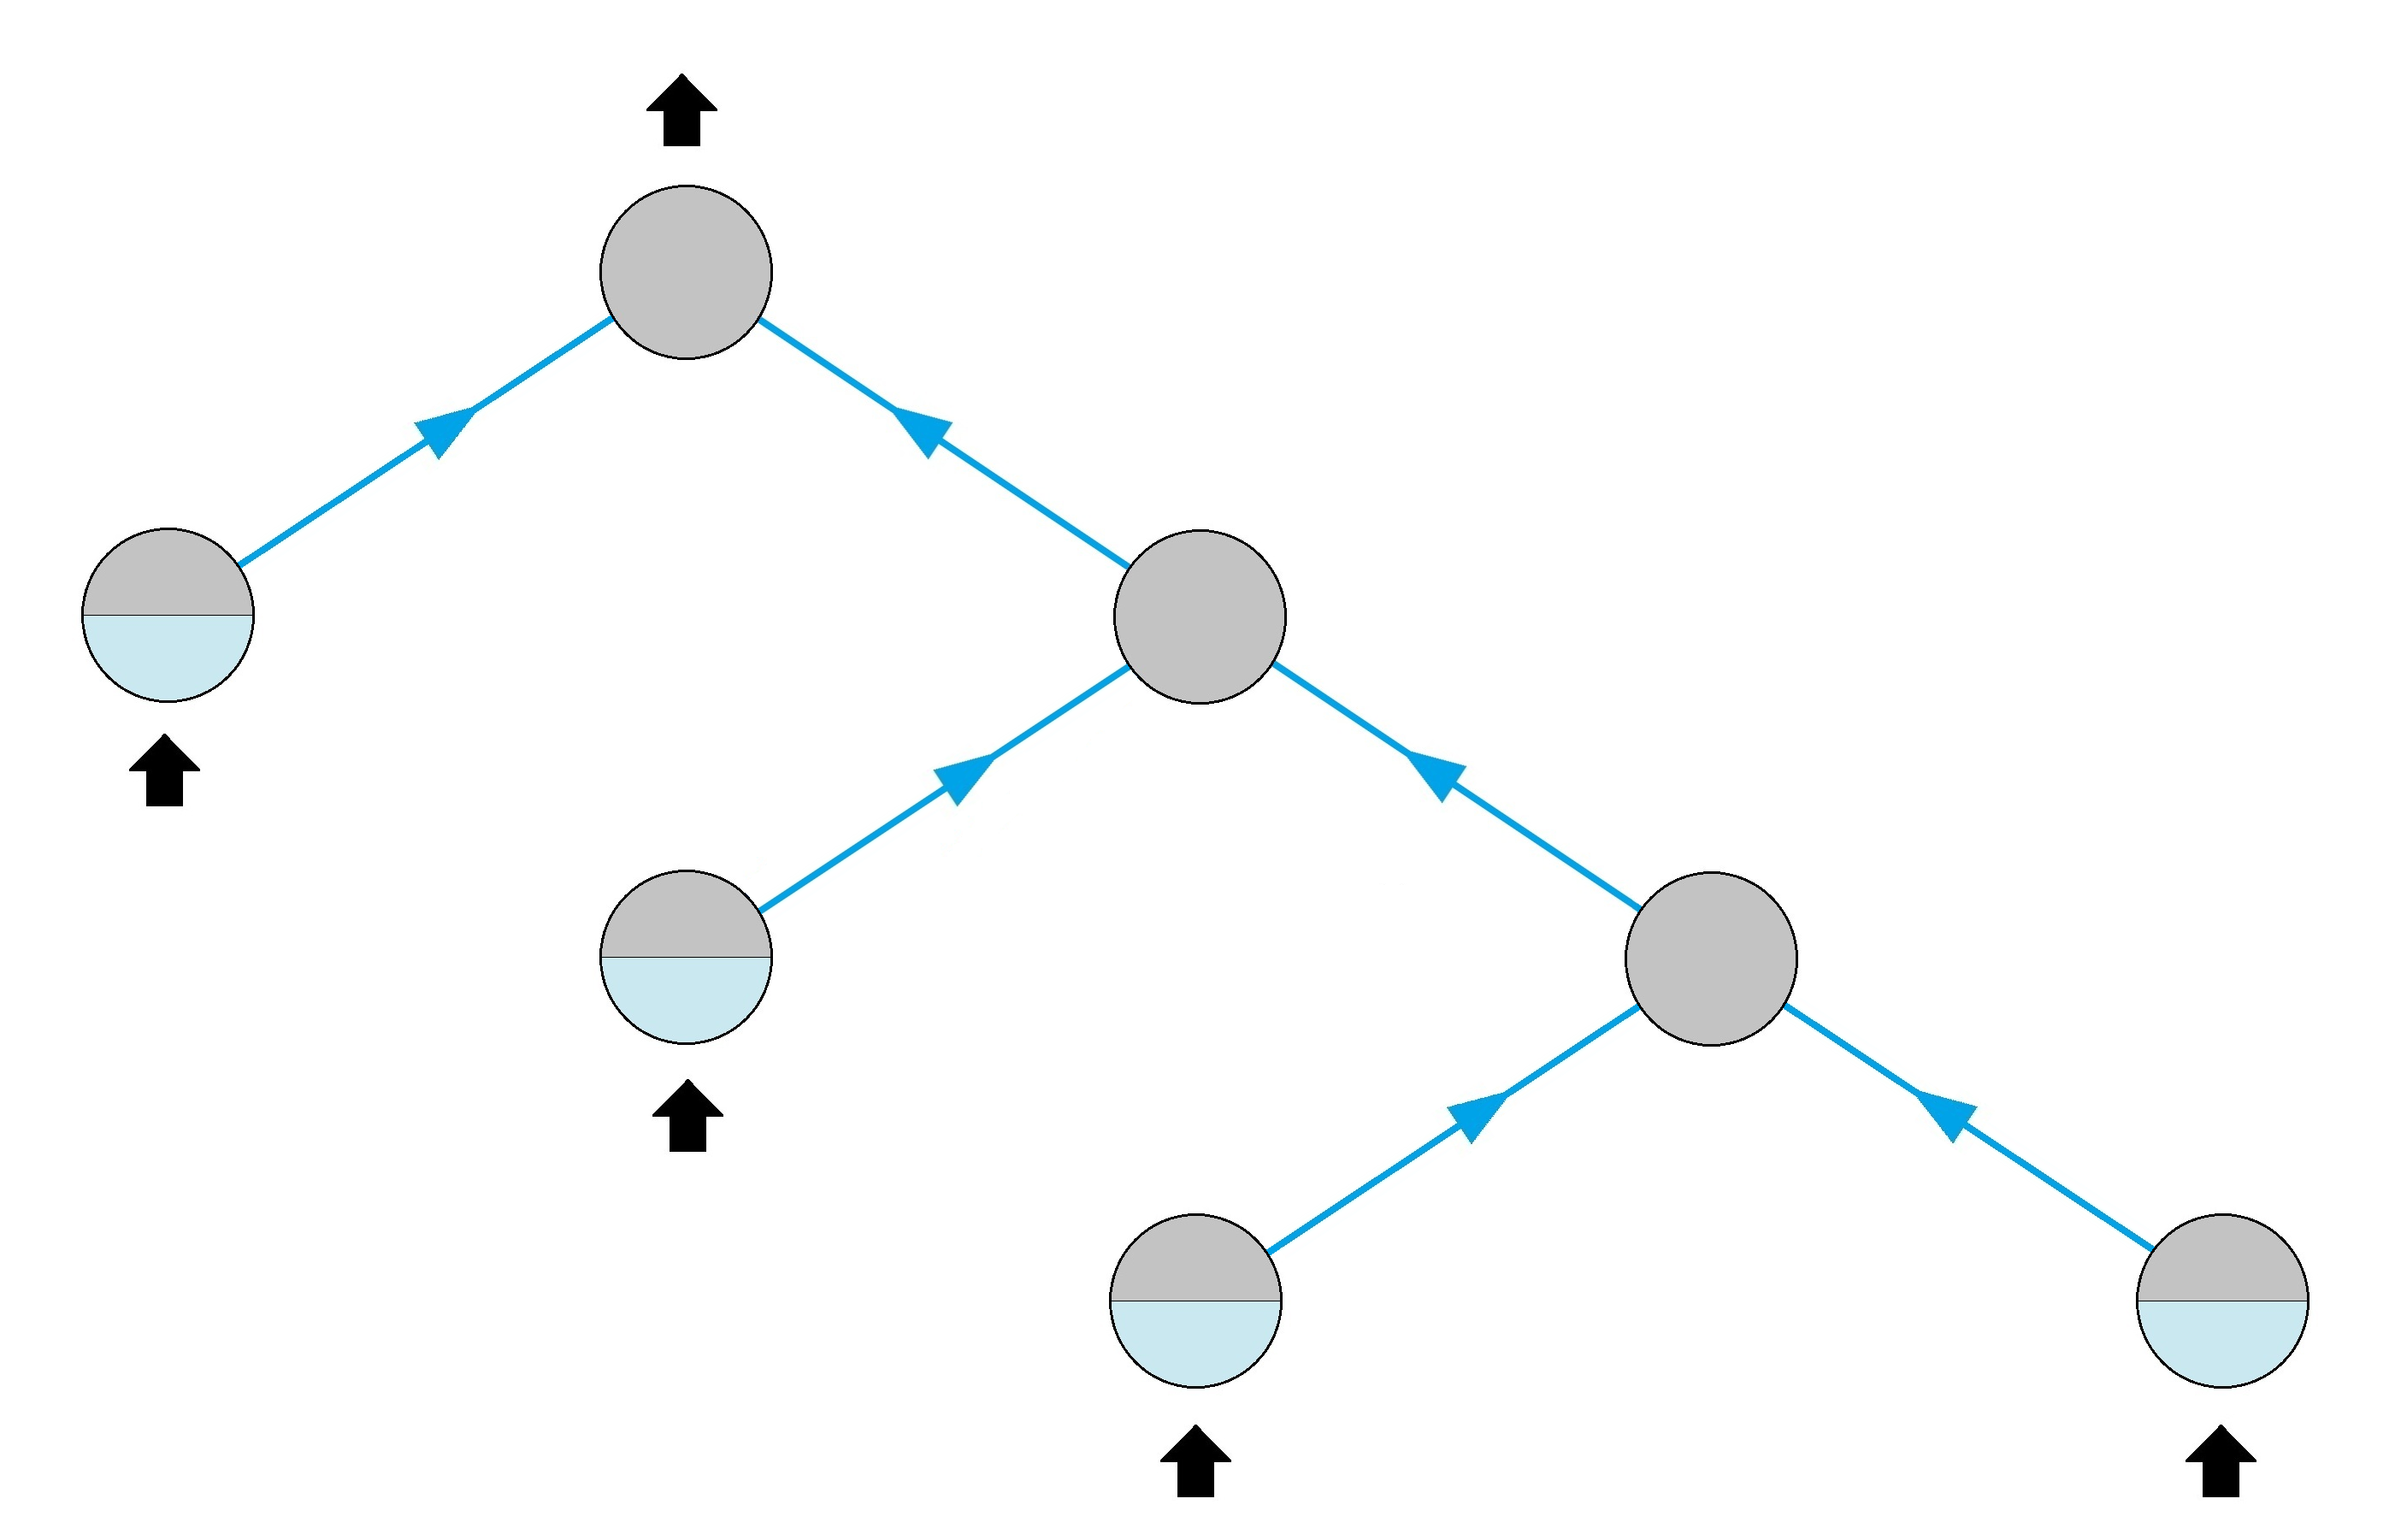
\includegraphics[width=\linewidth]{img/recursive/recursive_tree_potential_1.png}
        \caption{The tree representing an example recursive architecture of a potential recursive ensemble model that can be experimented with additional time. Each node is an instance of \texttt{RecursiveEnsembleNet}. The grey area represents an aggregator. The blue area represents an ensemble instance (e.g. \texttt{RecursiveStaticNCLEnsembleNet} instance) acting as a base learner. The blue arrows represent the data flows of predictions between \texttt{RecursiveEnsembleNet} instances. }
        \label{fig:recursive_tree_potential_1}
    \end{minipage}
    \hfill
    \begin{minipage}[t]{0.48\textwidth}
        \capstart
        \vspace{0pt}
        \centering
        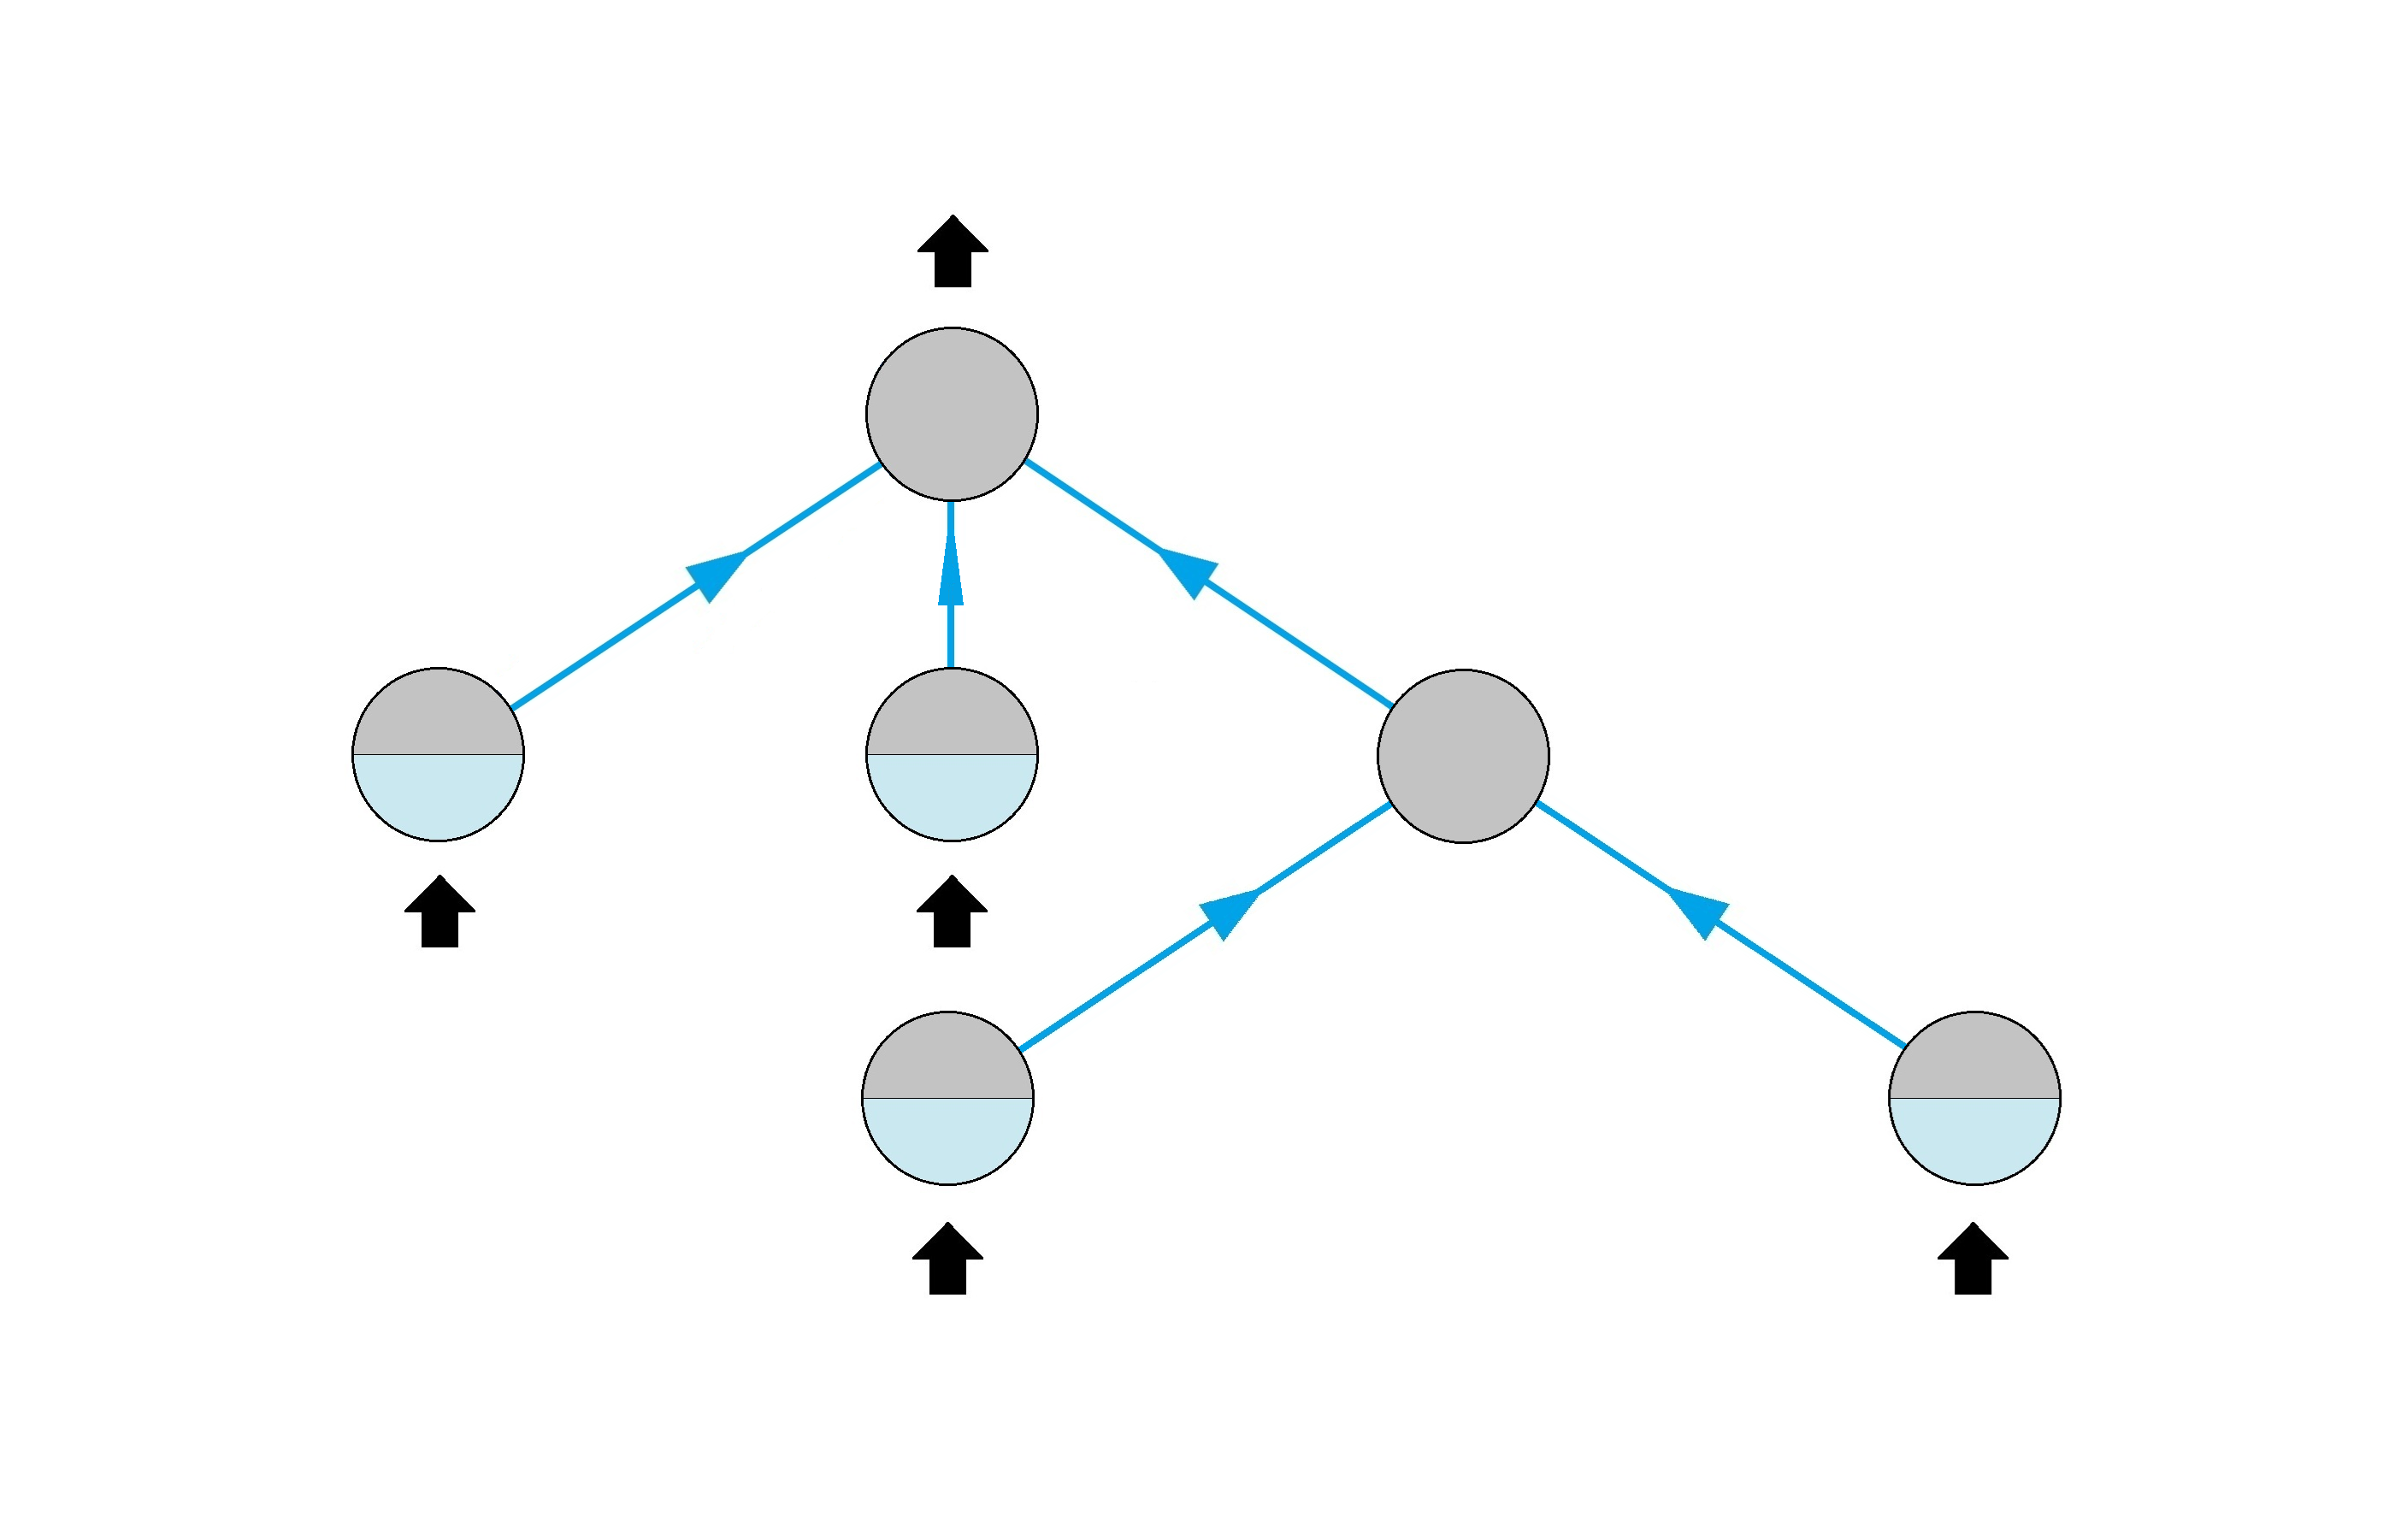
\includegraphics[width=\linewidth]{img/recursive/recursive_tree_potential_2.png}
        \caption{The tree representing an example recursive architecture of a potential recursive ensemble model that can be experimented with additional time. Each node is an instance of \texttt{RecursiveEnsembleNet}. The grey area represents an aggregator. The blue area represents an ensemble instance (e.g. \texttt{RecursiveStaticNCLEnsembleNet} instance) acting as a base learner. The blue arrows represent the data flows of predictions between \texttt{RecursiveEnsembleNet} instances. }
        \label{fig:recursive_tree_potential_2}
    \end{minipage}
\end{figure}